\documentclass[11pt,a4paper]{article}

\usepackage{main}
\usepackage{evaluation}

\renewcommand{\typedocument}{Évaluation}
\renewcommand{\classe}{3e}
\renewcommand{\titre}{Évaluation 1}

\begin{document}

\creertitre{\titre}

\vspace*{-0.5em}

\begin{center}
\textit{Durée : 30 minutes -- Calculatrice autorisée \\ Tous les exercices sont à faire sur la copie.}\\[1em]

\Large\textbf{Les météorites}
\end{center}

Une météorite est un fragment d'astéroïde, de taille très variable, qui s'est écrasée sur Terre à très grande vitesse. En 1960, fut découverte en Australie une météorite de \textbf{631 g} pour un volume de \textbf{90 cm\textsuperscript{3}}.

\exercice[]{Composition de la météorite}

\question[]{En précisant la formule utilisée, montrer par un calcul que la masse volumique $\rho$ de la météorite découverte en Australie a une valeur égale à \textbf{7,0 g/cm\textsuperscript{3}}.}

\vspace*{0.5em}

\fbox{\parbox{0.95\linewidth}{%
\uline{\textbf{Document 1 :} Classement des météorites}

La composition et la masse volumique d'une météorite permettent son classement en 3 catégories.

\begin{center}
\begin{tabular}{|l|c|p{7cm}|}
\hline
\rowcolor{headergrey}
\textbf{Catégorie} & \textbf{Masse volumique (g/cm\textsuperscript{3})} & \textbf{Composition} \\
    \hline
    Achondrite & Entre 3 et 3,5 & Calcium, Silicium et Magnésium \\
    \hline
    Chondrite & Entre 3,5 et 3,75 & Argile, calcium et silicium, teneur en métal inférieure à 35\% \\
    \hline
    Sidérite & Entre 4 et 7,5 & Fer, nickel (teneur inférieure à 5\%) \\
    \hline
\end{tabular}
\end{center}
}}

\question[]{\textbf{Indiquer} la catégorie à laquelle appartient cette météorite. \textbf{Justifier} votre réponse.}

\vspace*{0.5em}

Pour détecter la présence de fer dans une météorite, on plonge un fragment dans une solution acide. L'acide réagit avec le fer pour former des ions fer (II) Fe\textsuperscript{2+} et du dihydrogène H\textsubscript{2}.

\fbox{\parbox{0.95\linewidth}{%
\uline{\textbf{Document 2 :} Solutions de la vie quotidienne disponibles au laboratoire} 

\vspace{0.5em}
\begin{center}
\begin{tabular}{|l|c|}
    \hline
    \rowcolor{headergrey}
    \textbf{Nom de la solution} & \textbf{Valeur du pH} \\
    \hline
    Vinaigre & 2,6 \\
    \hline
    Eau savonneuse & 9,0 \\
    \hline
    Eau de Javel & 11,5 \\
    \hline
\end{tabular}
\end{center}
}}

\question[]{\textbf{Indiquer} le nom de la solution à utiliser pour détecter la présence de fer dans la météorite parmi les solutions proposées dans le document 2. \textbf{Justifier} votre réponse.}

\vspace*{1em}

\fbox{\parbox{0.95\linewidth}{%
\uline{\textbf{Document 3 :} Tests d'identification d'ions}

\vspace{0.1em}
\begin{center}
\begin{tabular}{|>{\centering\arraybackslash}m{3cm}|>{\centering\arraybackslash}m{4cm}|>{\centering\arraybackslash}m{4cm}|>{\centering\arraybackslash}m{4.5cm}|}
    \hline
    \rowcolor{headergrey}
    \textbf{Ion à identifier} & \textbf{Réactif utilisé} & \textbf{Formule de l'ion testeur} & \textbf{Couleur du précipité} \\
    \hline
    Fer (II) : Fe\textsuperscript{2+} & Hydroxyde de sodium (soude) & HO\textsuperscript{$-$} & Précipité vert \\
    \hline
    Fer (III) : Fe\textsuperscript{3+} & Hydroxyde de sodium (soude) & HO\textsuperscript{$-$} & Précipité orange \\
    \hline
    Calcium : Ca\textsuperscript{2+} & Oxalate d'ammonium & C\textsubscript{2}O\textsubscript{4}\textsuperscript{2$-$} & Précipité blanc \\
    \hline
    Chlorure : Cl\textsuperscript{$-$} & Nitrate d'argent & Ag\textsuperscript{$+$} & Précipité blanc qui noircit à la lumière \\
    \hline
\end{tabular}
\end{center}
}}

Pour prouver la présence de fer dans la météorite, il faut vérifier la présence d'ions fer (II) dans la solution obtenue après réaction avec l'acide.


\question[]{A l'aide du document 3, \textbf{indiquer} quel réactif utiliser pour vérifier la présence d'ions Fe\textsuperscript{2+} dans la solution.}

\question[]{\textbf{Indiquer} le résultat attendu de l'expérience si la météorite contient du fer. \textbf{Justifier} votre réponse.}

\exercice[]{Force gravitationnelle}

La Terre exerce une force attractive sur l'ensemble des corps qui l'entoure. Les météorites qui passent dans la zone d'influence de la Terre sont alors soumises à cette force gravitationnelle.

\question[]{\textbf{Recopier et compléter} les phrases suivantes avec la bonne proposition.}

\begin{enumerate}[label=\alph*)]
    \item La force gravitationnelle entre la Terre et la météorite est une action :
    \item[] $\triangleright$ à distance \hspace{2cm} $\triangleright$ de contact \vspace*{1.5em}
    \item La force gravitationnelle entre la Terre et la météorite s'exprime en :
    \item[] $\triangleright$ newton (N) \hspace{1cm} $\triangleright$ kilogramme (kg) \hspace{1cm} $\triangleright$ joule (J) \hspace{1cm} $\triangleright$ newton par kilogramme (N/kg) \vspace*{1.5em}
    \item L'intensité du \textbf{poids} de la météorite une fois tombée sur Terre se calcule à l'aide de la formule :
    \item[] $\triangleright$ $P = m \times g$ \hspace{1cm} $\triangleright$ $P = \frac{m}{g}$ \hspace{1cm} $\triangleright$ $P = U \times I$ \hspace{1cm} $\triangleright$ $P = m + g$ \vspace*{1.5em}
    \item L'interaction gravitationnelle entre la Terre et la météorite peut être représentée ainsi (écrire la lettre correspondant à la bonne figure) :
    \item [] a. \fbox{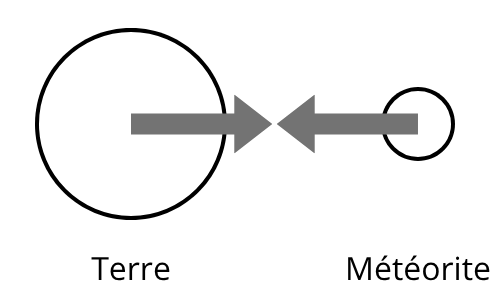
\includegraphics[width=4.1cm]{images/A.png}} \hspace{1cm} b. \fbox{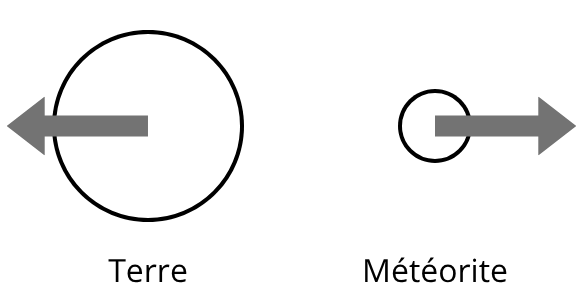
\includegraphics[width=5cm]{images/B.png}} \hspace{1cm} c. \fbox{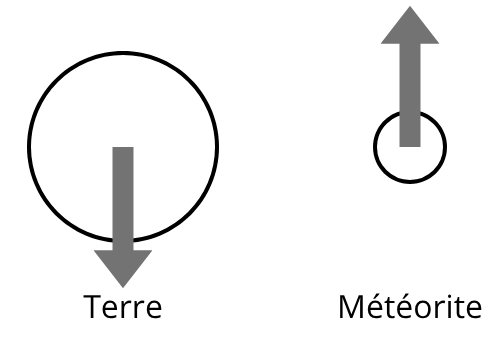
\includegraphics[width=3.8cm]{images/C.png}}
\end{enumerate}

\vspace*{2em}

\fbox{\parbox{0.95\linewidth}{%
\uline{\textbf{Document 4 :}} On rappelle que la valeur de la force gravitationnelle entre la Terre et la météorite est donnée par la formule :

\begin{center}
    $F = G \times \dfrac{m_T \times m}{d^2}$
\end{center}

\noindent Avec : \\
La constante gravitationnelle : $G = \SI{6,67e-11}{\N.m^2.kg^{-2}}$ \\
La masse de la Terre : $m_T = \SI{5,97e24}{kg}$ \\
La masse de la météorite : $m = \SI{0,631}{kg}$ \\
La distance entre la Terre et la météorite : $d = \SI{6,00e7}{m}$
}}

\vspace*{2em}

\question[]{\textbf{Calculer} la valeur de la force gravitationnelle exercée par la Terre sur la météorite découverte en Australie lorsqu'elle est à une distance de \textbf{60 000 km} du centre de la Terre. \textbf{Justifier} en détaillant le calcul en précisant les unités utilisées.}

\end{document}